%!TEX root = ../Main.tex

\chapter{Assignment 3.3}

\textbf{Create 2 modules that realize a producer and a consumer thread. The modules should be
	connected together using a sc\_fifo channel. Use the structure of a TCP package to simulate the
	data transmitted over the transmission (fifo) channel. The producer transmits a new TCP package
	with a random interval between 2-10 ms. The consumer thread must print the simulation time and
	sequence number each time a new TCP package is received. Use the TCP Header structure as
	described below with a total package size of 512 bytes. Inspiration can be found in the FifoFilter
	(Fork.h, when adding two consumers) example project.
}

For this problem two modules are implemented; a Consumer and a Producer module. 
A code snippet of the Costumer module is snippet below. 
The consumer module implements sc\_fifo\_in of the type <TCPHeader> because its supposed to read from the FIFO.

\section{Consumer.h}
\begin{lstlisting}
#pragma once
#include <systemc.h>
#include "TCPHeader.h"

SC_MODULE(Consumer)
{
sc_fifo_in <TCPHeader*> in;
TCPHeader *header;
SC_CTOR(Consumer)
{
SC_THREAD(ConsumerThread);
}

void ConsumerThread(void);
};
\end{lstlisting}


\section{Producer.h}
The same goes for the Producer module just vise versa it implements sc\_fifo\_out of the type <TCPHeader> because it’s supposed to write to the FIFO. The code snippet of the Producer module header file is pictured below.
\begin{lstlisting}
#pragma once
#include <systemc.h>
#include "TCPHeader.h"

SC_MODULE(Producer)
{
sc_fifo_out <TCPHeader*> out;
SC_CTOR(Producer)
{
SC_THREAD(ProducerThread);
}

void ProducerThread(void);
};
\end{lstlisting}





\section{TCPHeader.h}
In the header file for TCPheader the code snippet from the exercise was used as a template for the structure of the TCPheader. The implementation can be seen below. Comments in the code explain the implementation.

\begin{lstlisting}
#pragma once
#include <systemc.h>
#define PACKET_SIZE 512
#define DATA_SIZE (PACKET_SIZE-20)

class TCPHeader
{
sc_uint<16> SourcePort;
sc_uint<16> DestinationPort;
sc_uint<32> SequenceNumber;
sc_uint<32> Acknowledge;
sc_uint<16> StatusBits;
sc_uint<16> WindowSize;
sc_uint<16> Checksum;
sc_uint<16> UrgentPointer;
char Data[DATA_SIZE];

public:

// Empty constrtuctor
TCPHeader()
{

}

// Parametrized constructor
TCPHeader(sc_uint<16> SourcePort, sc_uint<16> DestinationPort, sc_uint<32> SequenceNumber, sc_uint<32> Acknowledge, sc_uint<16> StatusBits, sc_uint<16> WindowSize, sc_uint<16> Checksum, sc_uint<16> UrgentPointer, char Data[DATA_SIZE])
{
this->SourcePort = SourcePort;
this->DestinationPort = DestinationPort;
this->SequenceNumber = SequenceNumber;
this->Acknowledge = Acknowledge;
this->StatusBits = StatusBits;
this->WindowSize = WindowSize;
this->Checksum = Checksum;
this->UrgentPointer = UrgentPointer;
strcpy(this->Data, Data);
}

sc_uint<32> getSequenceNumber()
{
return SequenceNumber;
}

void setSequenceNumber(sc_uint<32> sn)
{
SequenceNumber = sn;
}

// Overload of '='-operator.
// Creates a new instance with matching attributes.
TCPHeader& operator=(
const TCPHeader& rhs
)
{
SourcePort = rhs.SourcePort;
DestinationPort = rhs.DestinationPort;
SequenceNumber = rhs.SequenceNumber;
Acknowledge = rhs.Acknowledge;
StatusBits = rhs.StatusBits;
WindowSize = rhs.WindowSize;
Checksum = rhs.Checksum;
UrgentPointer = rhs.UrgentPointer;
strcpy(Data, rhs.Data);
return *this;
}
// Overload of '=='-operator.
// Checks if all values are the same, in which case true is returned. Otherwise false is returned.
bool operator==(const TCPHeader& rhs)
const {
return SourcePort == rhs.SourcePort
&& DestinationPort == rhs.DestinationPort
&& SequenceNumber == rhs.SequenceNumber
&& Acknowledge == rhs.Acknowledge
&&StatusBits == rhs.StatusBits
&&WindowSize == rhs.WindowSize
&&Checksum == rhs.Checksum
&&UrgentPointer == rhs.UrgentPointer
&&strcmp(Data, rhs.Data);
}


//Definition of '<<'-operator and sc_trace.
friend ostream& operator<<(ostream& file, const TCPHeader& trans);
friend void sc_trace(sc_trace_file*& tf, const TCPHeader& trans, std::string nm);
};
\end{lstlisting}


\section{Producer.cpp}

If we look at the source file for the Producer which is pictured below. 
It generates a new TCPHeader called header, and write information about the package to the console, before writing the package to the FIFO. Then the sequence number is incremented before it waits for a random amount of time (between 2ms and 10ms). 

\begin{lstlisting}
#include "Producer.h"

sc_uint<16> SourcePort =  1;
sc_uint<16> DestinationPort = 2;
sc_uint<32> SequenceNumber = 1;
sc_uint<32> Acknowledge = 4;
sc_uint<16> StatusBits = 5;
sc_uint<16> WindowSize = 6;
sc_uint<16> Checksum = 7;
sc_uint<16> UrgentPointer = 8;
char Data[DATA_SIZE] = "Test Data";

void Producer::ProducerThread(void)
{
TCPHeader *header;
while (1)
{
// Generate new TCP header.
header = new TCPHeader(SourcePort, DestinationPort, SequenceNumber, Acknowledge, StatusBits, WindowSize, Checksum, UrgentPointer, Data);
cout << sc_time_stamp() << ": Producing" << endl;
cout << "Sending: " << endl << *header << endl << endl;

//Write to FIFO
out.write(header);

// Increment sequence number.
SequenceNumber++;

// Wait for 2-10 ms.
int waitTime = rand() % 10 + 2;
wait(waitTime, SC_MS);
}
}
\end{lstlisting}



\section{Consumer.cpp}
The consumer just reads from the FIFO, and writes out the sequence number on the received package to the console. 
\begin{lstlisting}
#include "Consumer.h"
#include "TCPHeader.h"

void Consumer :: ConsumerThread(void)
{
while (1)
{
// Blocking read from FIFO
header = in.read();
// Output timestamp and info about TCP package.
cout << sc_time_stamp() << " - Received TCP Package - Sequence number: " << (*header).getSequenceNumber() << endl << endl;
}
}
\end{lstlisting}



Below is a picture of the simulated result for the console. 
It matches the expected result. The sequence numbers match and the packages is being send in a random interval between 2ms and 10ms. 


\begin{figure}[H]
	\centering
	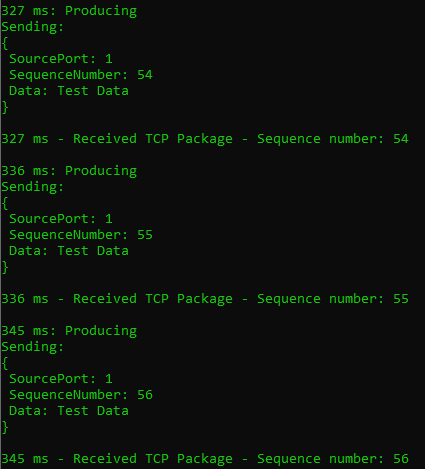
\includegraphics[width=\textwidth]{Images/ConsoleWindow3_3.png}
	\caption{A screenshot of the console}
	\label{fig:ConsoleWindow_3_3}
\end{figure}





